%
% path-finding
% @author Tobias Weber <tweber@ill.fr>
% @date 2021
% @license see 'LICENSE' file
%

\chapter{Path-finding Details and Implementation}
\label{ch:impl}

In this chapter we describe the individual steps of the strategy (see p. \pageref{sec:strategy}) in detail
and present an implementation in C++ \cite{Stroustrup2008, Stroustrup2018}. Specifically,
the latest version 20 of the C++ standard \cite{ISOCPP20} was employed in the creation of the software
together with the Boost C++ template libraries \cite{web_boost}. The source code for the implementation
can be found in the directory \lstinline|./src/core| together with the library routines in \lstinline|./src/libs|
of the repository at \url{https://code.ill.fr/scientific-software/takin/paths}. Stable versions of the
source code have furthermore been registered under the DOI \href{https://doi.org/10.5281/zenodo.4625649}{10.5281/zenodo.4625649}.

Section \ref{sec:tasmodel} is dedicated to modelling the triple-axis spectrometer (TAS), 
section \ref{sec:buildpath} discusses the steps involved in building up the instrument path, 
and section \ref{sec:exepath} focuses on executing the instrument motion along the path.
The graphical user interface is presented separately, namely in chapter \ref{ch:gui}.





% -----------------------------------------------------------------------------
% instrument model
% -----------------------------------------------------------------------------
\section{TAS instrument modelling}
\label{sec:tasmodel}

The instrument space comprising the triple-axis spectrometer, the walls and obstacles as well as the floor is modelled in
the class \lstinline[language=C++]|InstrumentSpace|. It also serves as high-level interface for loading and saving
the instrument geometry and states, signalling mechanisms for state changes using the publish-subscribe mechanism
via Boost.Signals2 \cite{web_boost_signals}, as well as checking the instrument for collisions.

The classes \lstinline[language=C++]|Instrument| and \lstinline[language=C++]|Axis| contain the actual instrument definition.
The spectrometer is modelled as a hierarchy of the three principal axes, namely monochromator, sample and analyser.
Each axis has three local coordinate systems, namely the rotation relative to the incoming and outgoing vector, respectively,
and an internal rotation which is decoupled from the other local rotations.
Geometrical objects are derived from the abstract, purely virtual class \lstinline[language=C++]|Geometry| and can be
coupled to any of these three local coordinate systems.
This makes it possible to model neutron-optical components attached to the either the incoming or outgoing path of the
neutron beam at the specific axis. It furthermore makes it possible to have components which rotate independently of
the axis.
Physically, the outgoing coordinate system is equal to the scattering angle, while the internal angle corresponds
to the crystal rocking angle (see Ch. \ref{ch:xtal}).
The transformation matrices corresponding to the three local coordinate systems are calculated as follows:

\begin{equation}
\begin{split}
	T_{\mathrm{in}}^{i} & \ =\  T_{\mathrm{out}}^{i-1} \cdot P^{i} \cdot R\left(\theta_{\mathrm{in}}^{i}\right), \\
	T_{\mathrm{int}}^{i} & \ =\  T_{\mathrm{in}}^{i} \cdot R\left(\theta_{\mathrm{int}}^{i}\right), \\
	T_{\mathrm{out}}^{i} & \ =\  T_{\mathrm{in}}^{i} \cdot R\left(\theta_{\mathrm{out}}^{i}\right).
\end{split}
\end{equation}

Here, $T_{\mathrm{in,\, int,\, out}}^{i}$ names the transformation matrices of the incoming, internal (decoupled) and outgoing
coordinate system of axis $i$, respectively.
$T_{out}^{i-1}$ is the outgoing transformation of the preceding instrument axis, or the identity if it is the first axis in the hierarchy.
$R\left(\theta_{\mathrm{in,\, int,\, out}}\right)$ are the corresponding rotation matrices and $P^i$ is the translation
of the local coordinate origin of the respective axis $i$.
The situation is depicted in Fig. \ref{fig:tas_axes}.


\begin{figure*}
	\begin{minipage}{0.45 \textwidth}
		\begin{center}
			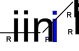
\includegraphics[width = 0.75 \textwidth]{figures/axis}
		\end{center}
	\end{minipage}
	%\hspace{1cm}
	\begin{minipage}{0.45 \textwidth}
		\begin{center}
			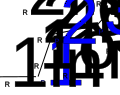
\includegraphics[width = 0.95 \textwidth]{figures/axes}
		\end{center}
	\end{minipage}
	\caption{Left panel: Local transformations for an axis. The symbols $R_{\mathrm{x}}^i$ are shorthands
	for the rotation matrices $R\left( \theta_{\mathrm{x}}^i \right)$, with $x = \left\{ \mathrm{in,\, int,\, out} \right\}$.
	$P^i$ is the point of origin for the axis.
	Right panel: Three coupled axes build up the triple-axis spectrometer, with axes 1, 2, and 3 naming the monochromator,
	the sample, and the analyser axis, respectively.
	\label{fig:tas_axes}}
\end{figure*}

% -----------------------------------------------------------------------------





% -----------------------------------------------------------------------------
% path building
% -----------------------------------------------------------------------------
\section{Path-building}
\label{sec:buildpath}

As discussed in chapter \ref{sec:tasrobot}, path-creation will be based on the angular configuration space
(as opposed to -- for example -- crystal configuration space). The top-level C++ class for creating the path
is named \lstinline[language=C++]|PathBuilder|. It mainly calls the low-level routines from the geometry
library situated in the directory \lstinline|./src/libs| of the source code repository.


\subsection{Angular configuration space}
As the obstacles do not have any geometrically primitive shape in angular configuration space, we iterate
through the configuration space on a two-dimensional grid and create a bitmap of allowed and forbidden
positions. The grid extends towards the scattering angles $2\theta_S \in \left[ -180^{\circ},\, 180^{\circ} \right]$ and monochromator angles of $2\theta_M \in \left[0^{\circ},\, 180^{\circ} \right]$, where, for the monochromator, we do
not the full angular range as this is not possible in real instruments which has the monochromator at a fixed position
and only scatters in one direction. The sample scattering angle, on the other hand, needs the full angular range as
scattering on both sides of the axis is done in practice.

To check for the allowed positions, the instrument model as described in sec \ref{sec:tasmodel} is moved to
each $\left( 2\theta_S,\, 2\theta_M \right)$ position on the grid and tested for collisions with the walls or with
itself. Even though the instrument model itself is a three-dimensional representation of the spectrometer, we
can nevertheless simplify the collision detection checks to a two-dimensional plane. The reason for this is
that all possible obstacles in the instrument path, for instance walls and pillars, are upright and do not have
any sloped angles. The same is true for the instrument itself.
The collision calculation on the two-dimensional grid is spread out on several processor cores using 
the \lstinline[language=C++]|thread_pool| \cite{web_boost_asio_threadpool} class from the 
Boost.Asio \cite{web_boost_asio} asynchronous input/output library.

With the given two-dimensional simplifications, we only need to distinguish three possible intersection tests for collisions: 
line-line intersections, line-circle intersections and circle-circle intersections. 
For efficiency, the actual calculations are only made if the corresponding geometrical objects lie within 
one another's axis-aligned bounding boxes \cite{web_aabb}.

\subsubsection*{Line-line intersections}
Given two lines $\left|x_1\right> + \lambda_1 \left|d_1\right>$ and $\left|x_2\right> + \lambda_2 \left|d_2\right>$, 
the line-line intersection can be calculated by setting their equations equal, namely as follows \cite{wiki_line_line_intersection}:
\begin{equation}
	\left|x_1\right> + \lambda_1 \left|d_1\right> \ =\ \left|x_2\right> + \lambda_2 \left|d_2\right>,
\end{equation}
\begin{equation}
	\left|x_1\right> - \left|x_2\right> \ =\  \lambda_2 \left|d_2\right> - \lambda_1 \left|d_1\right>,
\end{equation}
\begin{equation}
	\left|x_1\right> - \left|x_2\right> \ =\  D \cdot \left| \lambda \right>,
	\label{eq:line_line_inters}
\end{equation}
where, in the last step, the matrix $D$ is composed of the direction vectors in its columns, $D = \left( d_2 \ |\  -d_1 \right)$, 
and the vector $\left| \lambda \right>$ has the two individual line parameter $\lambda_1$ and $\lambda_2$ in its rows, $\left| \lambda \right> = \left( \lambda_2 \ |\  \lambda_1 \right)^T$.

For the given two-dimensional case, one can now directly solve for the $\lambda$s by left-multiplying with $D^{-1}$.
As the routine is also used by other code parts, we also include the general $n$-dimensional case in the implementation, 
determining the closest point between the two lines if no intersection exists.
This is done using the normal equation of the least-squares problem \cite[p. 793]{Arens2015}; 
the approximate version of Eq. \ref{eq:line_line_inters} thus reads \cite{wiki_line_line_intersection}: 
\begin{equation}
	D^T \left(\left|x_1\right> - \left|x_2\right>\right) \ =\  D^T D \cdot \left| \lambda \right>,
\end{equation}
\begin{equation}
	\left| \lambda \right> \ =\  \left( D^T D \right)^{-1} D^T \cdot \left( \left|x_1\right> - \left|x_2\right> \right).
\end{equation}

The intersection point (or the closest point) is thus be found by inserting the $\lambda$ parameters in the respective line equation. 
Testing for the intersection of line segments instead of infinite lines is done by keeping the $\lambda$ parameters inside a given range.

For an efficient handling of multiple line segment intersections, the decision for which lines to test for intersections is
performed using the line segment sweep algorithm from Ref. \cite[pp. 69-80]{FUH_geo2020} whose C++ implementation can be
found in the function \lstinline[language=C++]|intersect_sweep| of the file \lstinline|./src/libs/lines.h|.
We shortly summarise the algorithm and our implementation, following the description in \cite[pp. 69-80]{FUH_geo2020}:
\begin{enumerate}
	\item Possible events are kept in an event structure. Before the sweep, this is initialised with all the line segment
		endpoints. The structure itself is a priority queue which sorts its elements by their $x$ coordinate in ascending order.
		In the implementation we use the \lstinline[language=C++]|std::priority_queue| of the C++ standard library.
	\item The line sweep is performed by iteratively taking the top element from the event structure's priority queue until
		the latter is empty, in which case the algorithm terminates.
		Depending on the type of the current element on top of the event structure, the following actions are performed:
		\begin{itemize}
			\item If the current event is the left endpoint of a line segment, the newly encountered line segment is
				inserted into the sweep status structure and is tested for intersections against its preceding and succeeding
				line segment in the status structure. Potential intersections are inserted into the event structure.
				The sweep status structure sorts the line segments according to their $y$ order at the current $x$ position
				of the sweep line. It is implemented using Boost.Intrusive's \cite{web_boost_intrusive}
				AVL tree class \cite{web_boost_intrusive_avltree} and can be found in the file \lstinline|./src/libs/trees.h|.
			\item If the current event is the right endpoint of a line segment, the now inactive line segment is
				removed from the sweep status structure and its preceding and succeeding line segments are tested
				for intersection. A potential intersection is inserted into the event structure.
			\item If the current event is an intersection point, the involved line segments are reported as intersecting
				and, as they cross at this point, their order is flipped in the event structure.
				After the flip, the intersecting line segments are tested against intersection with their new neighbours
				and the possible intersection points are inserted into the event structure.
		\end{itemize}
	\item Repeat from step 2.
\end{enumerate}


\subsubsection*{Line-circle intersections}
As with the line-line intersection, we keep the problem general and directly look at the $n$-dimensional problem.
The intersection points between a line and an $n$-sphere are found by inserting the line equation 
$\left|p\right> = \left|x_1\right> + \lambda \left|d\right>$ into the sphere equation 
$\left< p-x_2 \ |\  p-x_2 \right> = r^2$, where $x_1$ names an arbitrary point on the line, $d$ its normalised 
direction vector, $x_2$ is the centre of the sphere/circle, and $r$ its radius \cite{wiki_line_sphere_intersection}.
The intersection points along the line are thus given by \cite{wiki_line_sphere_intersection}:
\begin{equation}
	\lambda \ =\ \left< x_2 - x_1 \  |\  d \right>
		\ \pm\ \sqrt{ \left< x_2 - x_1 \  |\  d \right>^2 
			+ r^2 - \left< x_2 - x_1 \ |\  x_2 - x_1 \right>}.
\end{equation}



\subsubsection*{Circle-circle intersections}
In this case we do not need the actual intersection points, so the calculation is restricted to calculation if
the circles overlap. This is the case when the distance of their centres $\left| x_1 \right>$ and $\left| x_2 \right>$ 
is less than the sum of their radii, $r_1$ and $r_2$, respectively:

\begin{equation}
	\left< x_2 - x_1 \ |\ x_2 - x_1  \right> \ \leq \ \left( r_2 + r_1 \right)^2.
\end{equation}



\subsection{Contour tracing}
Having determined a bitmap representation of allowed and forbidden regions in the angular configuration space,
we now need to trace the boundary contour between these regions.
To this end we use the radial sweep algorithm \cite{web_radial_sweep} whose implementation can be found
in the function \lstinline[language=C++]|trace_boundary| located in the file \lstinline|./src/libs/img.h|.

The radial sweep algorithm works as given below, following the descriptions in Ref. \cite{web_radial_sweep}:
\begin{enumerate}
	\item Scan the bitmap line by line and row by row until a forbidden region is found. 
		If the corresponding pixel has already been seen, continue. Otherwise mark it as start pixel.
	\item Set an arbitrary direction vector pointing to one of the eight neighbouring pixels.
	\item Rotate the direction vector in a given, fixed sense, i.e. either in an always clockwise or 
		always counter-clockwise fashion, until the pixel it points to is again inside a forbidden region.
		If a full rotation has been performed without hitting a new forbidden region, stop the algorithm.
	\item Increment the current pixel position using the newly found direction vector. 
		Set the new direction vector to point from the new pixel to the old one.
		Add the line connecting the old and the new pixel to the boundary.
	\item Repeat from step 3 until the start pixel is seen again (or no new direction vector is found).
\end{enumerate}


\subsection{Line-segment generation and simplification}


\subsection{Generation of convex regions}


\subsection{Calculation of the Voronoi diagram}
\label{sec:voronoi}


\subsection{Simplification of the Voronoi diagram}


% -----------------------------------------------------------------------------





% -----------------------------------------------------------------------------
% instrument motion
% -----------------------------------------------------------------------------
\section{Instrument movement}
\label{sec:exepath}


\subsection{Determination of the start and end coordinates}



\subsection{Calculation of Dijkstra's shortest path}
\label{sec:dijkstra}


% -----------------------------------------------------------------------------
